Flash loans do not enable anything new, it simply allows everyone to be able
to trade with large amounts of capital (for a single transaction). If you did
indeed possess a vast amount of wealth (if you are a whale) then flash loans are
not really of interest to you, you can already do the things it allows. With
that in mind, however, let's look at use cases for flash loans where most of them
are interesting because everyone can now do them, not just a select few with a
lot of capital. The following here is use-cases in which we can see the average
trader participating in due to the possibility presented by flash
loans\cite{attack}.

\begin{wrapfigure}{r}{5.5cm}
  \centering
  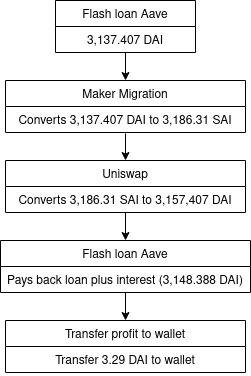
\includegraphics[width=.2\textwidth]{assests/Flash-loans-18-jan}
  \caption{A simplified figure showing the first arbitrage using flash loans.}
  \label{fig:firstArb}
\end{wrapfigure}
\paragraph{Arbitrage}
An asset's value is determined through supply and demand. So if there is a larger
supply of the asset than there is demand the price will go down, and if the
demand goes up, and the supply stays the same the price goes up. This is
reflected in the different DEX's, however they do not instantly synchronize. So
if one DEX trades an asset for a lower price than another, then there is
an \textit{arbitrage} opportunity. Arbitrage is the process of making profit off
of these prices difference. The way this is done, is by buying the asset at the
cheaper exchange, and then selling it again at the more expensive exchange. The
price differences will usually be small, so in order to make a significant
amount of money, you will need a great deal of capital. This is where flash
loans come in. Flash loans guarantees that the loans are paid back at the end of
the transaction, and arbitrage guarantees profit (if the trades back and forth
in the exchanges is instantaneous) therefore you could consider arbitrage
through flash loans risk-free, with the caveats that you do not count the
vulnerabilities of smart contracts and you do not consider gas-fees a risk.\\

The first arbitrage, using flash loans, was reported by Camilla Russo
on twitter\footnote{Camilla Russo twitter post
  \url{https://twitter.com/CamiRusso/status/1218640871048056832}}. We
have illustrated a walkthrough of the arbitrage in figure
\ref{fig:firstArb}, where we can see that the arbitrage opportunity
lies in the exchange rate of Uniswap not matching the migration on
MakerDAO.

\paragraph{Wash Trading} When trading it is important to keep an eye
on the trends of the market, what asset is frequently traded, how much
of it, and why. Wash trading is the process of creating an artificial
trend by buying and selling an asset thereby increasing the volume at
which the asset is traded which will attract investors. This practice
has been banned (in the USA) on the centralized markets since
1936. While we do not condone this practice it is undeniable a
use-case for flash loans, since you can with no significant capital greatly
increase the trade volume of an asset, and thereby manipulate the
market.

\paragraph{Collateral Swapping} Lots of DeFi protocols allows you to
put up collateral for loans, however, there could be reasons for you
wanting to change that collateral for example if your collateral is in
ETH and the value of ETH declines, then you might want to swap it for
DAI but you might have taken out loans against this collateral, so you
do not have the capital to pay out your collateralized position and
take out a new one in a different asset. With flash loans this becomes
easy, you would loan the amount you need to pay out your position, swap
that capital to the asset you want as the new collateral, take out a
new collateralized position, and finally pay back the loan.

\paragraph{Liquidation auction} When a CDP (Collateralized Debt Position) is
opened at e.g. Maker, they require you to put up ETH as collateral for the loan
you take in DAI. If ETH falls in value enough, you will end up below a certain
threshold (150\%). If this occurs, your collateral will be auctioned off, to
cover your debt with an added penalty fee. To earn money from this
using flash loans, one can take a flash loan and buy collateral at an auction.
Because the collateral should still be worth more than 100\% of the debt, you
should end up with a profit, that can then be used to pay back the flash loan.
There is relatively little risk, as you at most end up losing the gas fees.
